\chapter{Experiments and Results}\label{ch:experiments}

This chapter reports the empirical evaluation of the three
proposed mechanisms on the cross-architecture transfer matrix
defined in Chapter~\ref{ch:proposed}. The matrix is the principal
artefact: the chapter does not lead on any single test character
error rate, but on the pattern across the matrix and on the
mechanism-prior alignment criterion that the pattern supports.
Section~\ref{sec:experiments:framework} states the experimental
framework, including the probes, the evaluation conventions, and
the matched training budget. Section~\ref{sec:experiments:summary}
aggregates the empirical results into a single table.
Sections~\ref{sec:experiments:transfer} through
\ref{sec:experiments:synthesis} take one row of the argument at a
time.

\section{Experimental framework}\label{sec:experiments:framework}

The empirical evaluation rests on three probes selected for the
expressivity axis each one exercises rather than for
aggregate-score competitiveness. The framework is summarised in
this section; complete hyperparameter tables, dataset construction
details, and the hardware environment live in
Appendix~\ref{app:experimental-setup}.

\paragraph{Probes and data preparation.} The principal probe is
LibriSpeech train-clean-100~\cite{panayotov2015librispeech},
$100$~hours of audiobook-source read English speech preprocessed
into $80$-mel log-spectrograms with $25$~ms window and $10$~ms
hop, followed by $2\times$ acoustic subsampling that brings
post-frontend sequence length to $T \le 500$ at the
phoneme-to-syllable scale relevant to the axis-1 deficit. The
cross-distribution probe is a $100$-hour balanced subset of
Common Voice English~\cite{ardila2019commonvoice} sampled
stratified by speaker so that no speaker appears in more than one
of the train, dev, or test partitions, with the cumulative
duration matching the LibriSpeech budget within rounding. Both
acoustic probes share the same $29$-symbol character vocabulary
(twenty-six lowercase letters, the apostrophe, the space
character, and a dedicated CTC blank token). The synthetic axis-2
probe is the Multi-Query Associative Recall benchmark of
\citet{arora2023zoology} with the canonical sequence-length sweep
$T \in \{64, 256, 1024\}$ and the matching stored-pair counts
$K \in \{16, 64, 256\}$ that grow with $T$ to keep the difficulty
parameter $K / d$ meaningful at every length. The synthetic probe
uses two disjoint $8192$-token vocabularies for keys and values.
Table~\ref{tab:librispeech-vs-cv} summarises the pre-experimental
comparison between the two acoustic probes that motivates the
cross-distribution validation of
Section~\ref{sec:experiments:cv}; the broader acoustic variance of
Common Voice along speaker, accent, and recording-condition axes
is identified as a probe property prior to any experiment on the
proposed mechanisms.

\begin{table}[!htbp]
\centering
\small
\caption[LibriSpeech clean-100 versus Common Voice English 100h]{
Pre-experimental comparison of the two acoustic probes along the
axes that motivate the cross-distribution validation of
Section~\ref{sec:experiments:cv}. Numbers and qualitative
descriptors are taken from~\citet{panayotov2015librispeech} for
LibriSpeech and~\citet{ardila2019commonvoice} for Common Voice;
subset-construction details for the $100$~h Common Voice partition
are recorded in Appendix~\ref{app:setup:cv}.}
\label{tab:librispeech-vs-cv}
\setlength{\tabcolsep}{4pt}
\renewcommand{\arraystretch}{1.2}
\begin{tabularx}{\linewidth}{@{}p{3.2cm} X X@{}}
\toprule
\textbf{Property} & \textbf{LibriSpeech train-clean-100} & \textbf{Common Voice English 100h} \\
\midrule
Source protocol
  & Audiobook reading from LibriVox
  & Volunteer crowd-sourced single-read contribution \\
\addlinespace
Total duration
  & $100.6$~h
  & $100$~h, balanced subset of the validated split \\
\addlinespace
Speaker count
  & $251$ speakers
  & Several thousand contributors in the validated split, sampled stratified so no speaker appears in more than one of train, dev, test \\
\addlinespace
Accent annotation
  & Not provided
  & Annotated across multiple regional varieties of English \\
\addlinespace
Recording conditions
  & Studio-grade, single read protocol
  & Heterogeneous; volunteer microphones, varied recording environments \\
\addlinespace
Vocabulary head
  & $29$-character CTC head
  & $29$-character CTC head (shared with LibriSpeech) \\
\bottomrule
\end{tabularx}
\end{table}

\paragraph{Evaluation framework.} The acoustic probes report
character error rate under full-utterance greedy connectionist
temporal classification decoding~\cite{graves2006ctc} with no
language-model rescoring and no beam search. The choice removes
two sources of variance from the mechanism attribution: the
autoregressive sampling noise that beam search and language-model
rescoring introduce, and the architectural confound of an
external decoder whose contribution to the metric overlaps with
what the encoder mechanism is meant to deliver. The omission is
deliberate rather than incidental, since either decoder addition
would introduce a decoder-architecture-bias confound with the
encoder-level mechanism attribution that is the chapter's
principal claim. The synthetic
probe reports per-sequence accuracy under a verdict convention
shared with the Zoology study: a cell PASSes when per-sequence
accuracy reaches $0.99$ at the early-stopping point, FAILs when
accuracy stays at or near zero with the loss flat near the
initialisation level, and PARTIALs in the intermediate band. The
chunked-streaming evaluation, reported in
Appendix~\ref{app:diagnostics:chunked}, supplements the
full-utterance acoustic test by isolating the short-window regime
in which the recurrent state has not accumulated long-context
information. The framework is justified by the matrix-as-artefact
position: clean per-cell attribution at the architectural level
is preferred over decoder-coupled aggregate scores, since the
chapter's empirical claim is the pattern of relative gains rather
than any single absolute metric.

\paragraph{Training budget and parameter match.} Every
LibriSpeech and Common Voice cell is trained under a locked
50-epoch matched budget with AdamW, peak learning rate
$3 \times 10^{-4}$, cosine schedule with $1000$-step linear
warmup, and SpecAugment LD policy~\cite{park2019specaugment}; the
synthetic probe uses a step-based budget of up to $30\,000$
training steps with early stopping when per-sequence accuracy
reaches $0.999$ on a held-out validation batch. Full
hyperparameters are tabulated in
Appendix~\ref{app:experimental-setup}. The encoder configuration
at the 7M scale is $d_{\text{model}} = 256$, six layers,
$H = 4$ heads, head dimension $64$; at the 14M scale the layer
count doubles to twelve with the other widths unchanged. All
mechanism cells within the same scale are parameter-matched to
within approximately two percent of the vanilla baseline of the
same architecture, with the largest mechanism overhead introduced
by the Damped Harmonic Oscillator on RWKV-6 ($+0.075$~M out of
$7.74$~M at 7M, $+0.224$~M out of $13.56$~M at 14M); per-cell
parameter counts are reported in Appendix~\ref{app:results}.
Reported gains are not bought by parameter inflation.

All cells are trained at single seed. The matched 50-epoch budget
across 65 cells exhausts the available compute for this thesis,
and the directional coherence of the across-matrix pattern
provides aggregate statistical confidence that offsets the
variance of any individual cell. The empirical noise floor on
test character error rate between matched re-runs at the codebase
configuration is approximately $\sigma \approx 0.0014$, estimated
from prior matched-budget runs. The chapter applies the
convention that a per-cell $\Delta$ at $|\Delta| > 5\sigma$ is in
the BREAK band, $|\Delta| \le 2\sigma$ is marginal, and
intermediate values are productive but not BREAK.

\section{Aggregated empirical summary}\label{sec:experiments:summary}

Table~\ref{tab:results:aggregated} aggregates the LibriSpeech test
character error rate of every reported configuration in the
matrix. Per-cell breakdowns including dev character error rate,
parameter counts, the Common Voice cross-distribution comparison,
the Multi-Query Associative Recall length sweep, and the
chunked-streaming evaluation live in
Appendix~\ref{app:results}; the supplementary diagnostic figures
and the operator-level bidirectional comparison live in
Appendix~\ref{app:diagnostics}.

\begin{table}[!htbp]
\centering
\small
\caption[Aggregated test character error rate across the
matrix]{Aggregated test character error rate on LibriSpeech
test-clean across the cross-architecture transfer matrix at the
matched 50-epoch budget. Each row is a single
(architecture, mode, scale) configuration; non-vanilla cells give
test CER followed by the relative reduction over the matched
vanilla baseline in parentheses. The composition column reports
the pre-registered composition for each architecture
(CVD~$\times$~MSDC on RWKV-6 and Mamba-2; DHO~$\times$~MSDC on
Linear Attention). Bold values mark the matrix ceiling on the
14M Mamba-2 row.}
\label{tab:results:aggregated}
\setlength{\tabcolsep}{4pt}
\renewcommand{\arraystretch}{1.20}
\begin{tabularx}{\linewidth}{@{}X r r r r r@{}}
\toprule
\textbf{Configuration} &
\textbf{Vanilla} & \textbf{MSDC} & \textbf{CVD} &
\textbf{DHO} & \textbf{Composition} \\
\midrule
RWKV-6 causal 7M       & 0.1049 & 0.0788 ($-25\%$) & 0.1007 ($-4\%$) & 0.0989 ($-6\%$) & 0.0785 ($-25\%$) \\
Mamba-2 causal 7M      & 0.1036 & 0.0825 ($-20\%$) & 0.0958 ($-8\%$) & 0.1006 ($-3\%$) & 0.0795 ($-23\%$) \\
LA causal 7M           & 0.1879 & 0.1409 ($-25\%$) & 0.1714 ($-9\%$) & 0.1198 ($-36\%$) & 0.0999 ($-47\%$) \\
\addlinespace
RWKV-6 causal 14M      & 0.1103 & 0.0751 ($-32\%$) & 0.1051 ($-5\%$) & 0.1077 ($-2\%$) & 0.0746 ($-32\%$) \\
Mamba-2 causal 14M     & 0.0827 & \textbf{0.0631} ($-24\%$) & 0.0728 ($-12\%$) & 0.0781 ($-6\%$) & \textbf{0.0618} ($-25\%$) \\
LA causal 14M          & 0.1359 & 0.0969 ($-29\%$) & 0.1300 ($-4\%$) & 0.0947 ($-30\%$) & 0.0786 ($-42\%$) \\
\addlinespace
RWKV-6 LION-S 7M       & 0.0859 & 0.0750 ($-13\%$) & 0.0852 ($-1\%$) & 0.0740 ($-14\%$) & 0.0747 ($-13\%$) \\
Mamba-2 LION-S 7M      & 0.0853 & 0.0833 ($-2\%$) & 0.0849 ($-1\%$) & 0.0825 ($-3\%$) & 0.0805 ($-6\%$) \\
LA LION-LIT 7M         & 0.2951 & 0.1404 ($-52\%$) & 0.3194 ($+8\%$) & 0.1042 ($-65\%$) & 0.0961 ($-67\%$) \\
LA LION-S 7M           & 0.1381 & 0.1154 ($-16\%$) & 0.1311 ($-5\%$) & 0.0988 ($-28\%$) & 0.1129 ($-18\%$) \\
\bottomrule
\end{tabularx}
\end{table}

The relative reductions in
Table~\ref{tab:results:aggregated} are scaled by each row's
vanilla baseline; the deficit-proportional ordering claim of
Section~\ref{sec:experiments:transfer} is argued in absolute
$\Delta$ terms because baseline differences shift the relative
ordering on some MSDC cells.

The matrix populates the mechanism-prior alignment criterion of
Chapter~\ref{ch:proposed} in three signatures across the family.
On the Multi-Scale Depthwise Convolution row, the gain orders
with the deficit map of Section~\ref{sec:backbones:deficit}: the
backbone with no native local mixing receives the largest gain.
On the Damped Harmonic Oscillator row, the same deficit map
predicts a structural BREAK on the architecture whose vanilla
transition admits no native attenuation and no native phase, and
a near-null on the architecture whose selective transition
absorbs the block-complex extension under the LibriSpeech
distribution. On the Chunked Value Decorrelation row, the
transfer is asymmetric across the family, and the LION mode
contains the single counter-example to productive transfer in
the matrix; the structural reading of this counter-example is
the subject of Section~\ref{sec:experiments:lion}. The
remaining sections present each row of the argument with the
corresponding figure.

\section{Transfer pattern on LibriSpeech}\label{sec:experiments:transfer}

The transfer pattern of each mechanism across the three causal
backbones at 7M and 14M is visualised in
Figure~\ref{fig:f1-transfer-pattern}; the deficit-proportional
ordering of the Multi-Scale Depthwise Convolution row is
isolated in Figure~\ref{fig:f2-deficit-ordering}. The three
mechanisms produce three structurally distinct signatures in
the matrix, predicted in each case from the architecture-deficit
map of Section~\ref{sec:backbones:deficit}.

\begin{figure}[!htbp]
\centering

\includegraphics[width=0.9\linewidth]{figures/chapter5/F1_transfer_pattern_matrix.pdf}
\caption[Transfer-pattern matrix]{Test character error rate
$\Delta$ versus the architecture-mode-scale vanilla baseline,
faceted by access mode and parameter scale. Rows index
architecture; columns index mechanism. Blue indicates a helpful
$\Delta$, red indicates a harmful $\Delta$, and the colour
intensity scales with magnitude. The single red cell is the
LA LION-LIT~$\times$~CVD configuration at the 7M scale.}
\label{fig:f1-transfer-pattern}
\end{figure}

\paragraph{MSDC universal, deficit-proportional.} The mechanism
transfers productively across all three causal backbones at
both scales. The ordering of $\Delta$ matches the share of
axis-1 coverage each backbone already had: Linear Attention,
with no native local mixing, receives the largest gain
($\Delta = -0.0470$ at 7M, $-0.0390$ at 14M); RWKV-6, whose
Time-Mix block carries a single-step data-dependent token
shift, receives an intermediate gain ($-0.0261$ at 7M,
$-0.0352$ at 14M); Mamba-2, whose vanilla path includes a
native short convolution at $k = 4$, receives the smallest gain
($-0.0211$ at 7M, $-0.0196$ at 14M). The LA $>$ RWKV-6 $>$
Mamba-2 ordering is reproduced at both scales, and the gain on
RWKV-6 grows with capacity, indicating that the mechanism
recovers more of the architectural deficit at higher scale
rather than saturating. The relative-reduction column of
Table~\ref{tab:results:aggregated} differs from this absolute
ordering at 14M, where MSDC delivers $-32\%$ on RWKV-6 against
$-29\%$ on LA: the discrepancy reflects the difference in
vanilla baselines ($0.1103$ on RWKV-6 versus $0.1359$ on LA at
14M). The deficit-proportional claim is argued in absolute
$\Delta$ terms throughout the chapter, since the
architecture-deficit map of
Section~\ref{sec:backbones:deficit} predicts absolute headroom
rather than fractional reduction.

\begin{figure}[!htbp]
\centering
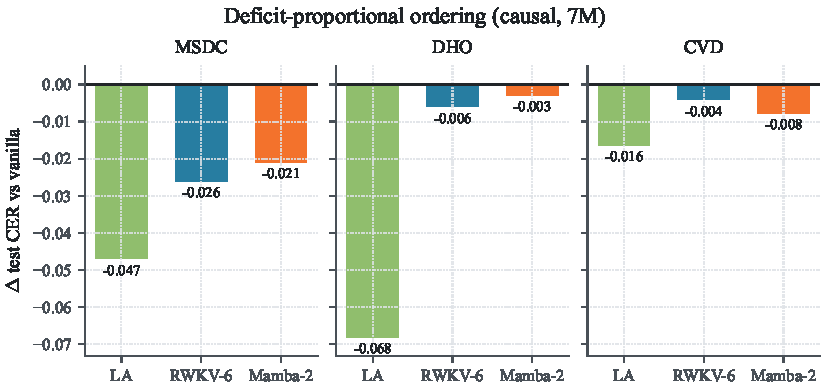
\includegraphics[width=0.9\linewidth]{figures/chapter5/F2_deficit_proportional_ordering.pdf}
\caption[Deficit-proportional ordering of MSDC]{Test $\Delta$ of
the Multi-Scale Depthwise Convolution mechanism across the
three causal backbones at 7M and 14M. The ordering LA $>$
RWKV-6 $>$ Mamba-2 reproduces at both scales and matches the
architecture-deficit map of
Section~\ref{sec:backbones:deficit}.}
\label{fig:f2-deficit-ordering}
\end{figure}

\paragraph{DHO: BREAK on Linear Attention, near-null on Mamba-2.}
The Damped Harmonic Oscillator extends the real-diagonal
transition with the block-complex closure of
Section~\ref{sec:proposed:dho}. Its predicted reach is largest
on the architecture whose vanilla transition admits no native
attenuation and no native phase, and smallest on the
architecture whose selective scalar transition absorbs the
block-complex extension under the LibriSpeech distribution. The
matrix matches the prediction: on Linear Attention at 7M
causal, $\Delta = -0.0681$ (a $36\%$ relative reduction over
the LA vanilla baseline), the largest single-mechanism gain in
the matrix, with the BREAK pattern preserved at 14M
($-0.0412$); on Mamba-2 at 7M causal, $\Delta = -0.0030$, near
the noise floor of the matched-budget evaluation, and similarly
near-null at 14M ($-0.0046$); on RWKV-6, whose per-channel
data-dependent decay already covers the attenuation component,
$\Delta = -0.0061$ at 7M and $-0.0026$ at 14M.
Section~\ref{sec:experiments:cv} returns to the Mamba-2
near-null and shows that the absorption is task-prior modulated
rather than absolute.

\paragraph{CVD: asymmetric.} The Chunked Value Decorrelation
transfers asymmetrically across the family. On Linear Attention
at 7M causal, $\Delta = -0.0165$, the largest CVD gain in the
matrix; on Mamba-2, $\Delta = -0.0078$; on RWKV-6,
$\Delta = -0.0042$. The ordering inverts the natural-home-in-
attention prior, since the value-decorrelation principle
descends from a softmax-attention construction
(Section~\ref{sec:primitives:cvd}) and might be expected to
transfer most strongly to the family member whose recurrence
is closest to softmax attention. The matrix instead places the
largest gain on the no-decay backbone. The LION-mode reading of
this asymmetry is the subject of
Section~\ref{sec:experiments:lion}.

\section{Cross-scale persistence and LION
mode}\label{sec:experiments:lion}

The mechanism transfer pattern of
Section~\ref{sec:experiments:transfer} preserves across the
7M-to-14M scaling step on the causal matrix; on the LION
bidirectional matrix at 7M, the same pattern reproduces
conditional on a structural prerequisite identified in this
section. Figure~\ref{fig:f5-cross-scale} reports the cross-scale
persistence; Figure~\ref{fig:f7-causal-lion} reports the
causal-versus-LION mode comparison.

\begin{figure}[!htbp]
\centering
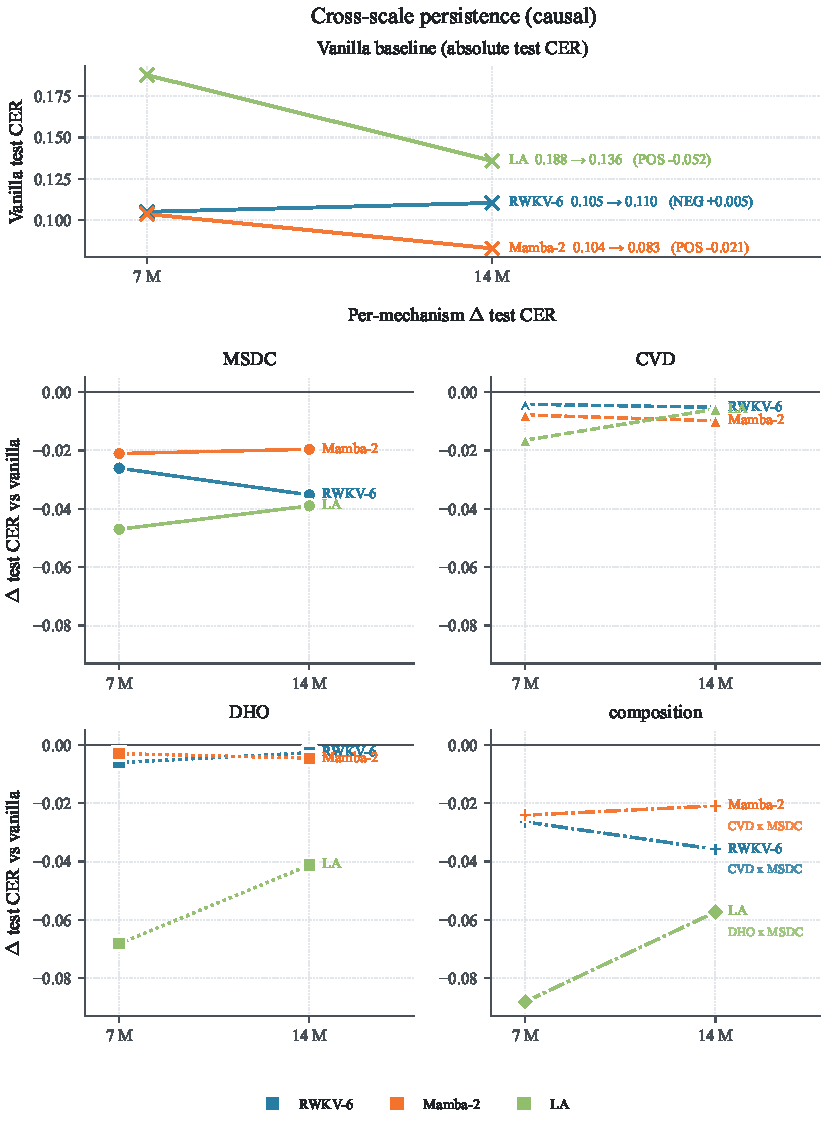
\includegraphics[width=0.9\linewidth]{figures/chapter5/F5_cross_scale_persistence.pdf}
\caption[Cross-scale persistence at 7M and 14M]{Test character
error rate at the 7M and 14M scales for every causal-mode cell
of the matrix. Lines connect the same architecture-mechanism
pair across scales; positive slope indicates a regression on
scaling, negative slope indicates an improvement. The 14M
Mamba-2 MSDC and CVD~$\times$~MSDC cells form the matrix
ceiling at $0.0631$ and $0.0618$ respectively.}
\label{fig:f5-cross-scale}
\end{figure}

\paragraph{Cross-scale persistence.} The MSDC mechanism gain
preserves on Mamba-2 ($\Delta = -0.0211 \to -0.0196$) and Linear
Attention ($-0.0470 \to -0.0390$) and grows on RWKV-6
($-0.0261 \to -0.0352$). The LA $>$ RWKV-6 $>$ Mamba-2 ordering
predicted by the deficit map of
Section~\ref{sec:backbones:deficit} preserves at both scales.
The CVD and DHO mechanisms preserve their causal-mode
signatures across scale as well, with CVD asymmetric and DHO
BREAK on Linear Attention and near-null on Mamba-2. No mechanism
exhibits a ranking inversion under the 7M-to-14M scaling step;
the conditional 30M scale is dropped from scope on this basis.
The matrix ceiling at 14M is the Mamba-2 CVD~$\times$~MSDC
composition at $0.0618$, with the Mamba-2 MSDC single-mechanism
cell at $0.0631$ slightly above.

\begin{figure}[!htbp]
\centering
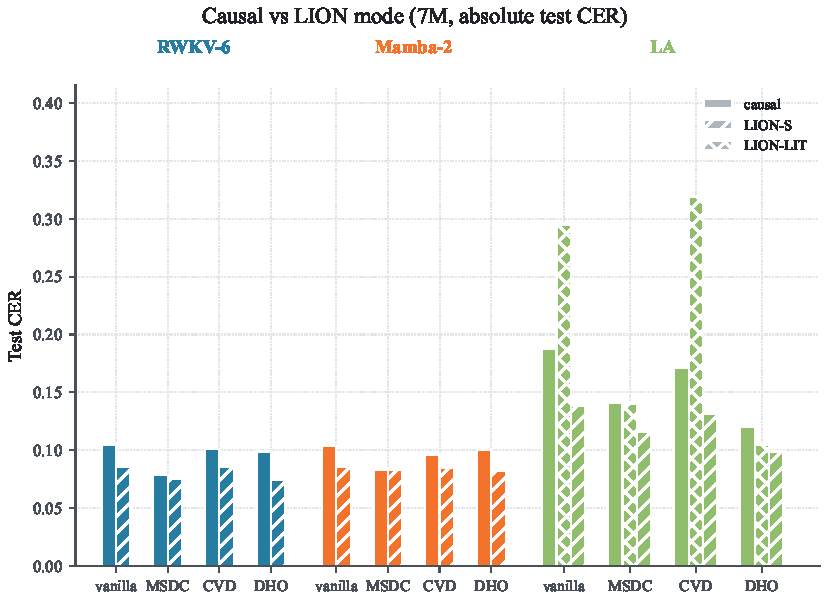
\includegraphics[width=0.9\linewidth]{figures/chapter5/F7_causal_lion_mode.pdf}
\caption[Causal versus LION mode comparison]{Test character
error rate per (architecture, mechanism) pair in causal mode and
in LION bidirectional mode at 7M. Linear Attention is reported
in two LION variants: LION-LIT, the natural mapping
per~\citet{afzal2025linear} Table~1 (no decay, $\lambda = 1$),
and the controlled LION-S deployment, which adds a per-token
sigmoid decay that is not present in the underlying causal
backbone.}
\label{fig:f7-causal-lion}
\end{figure}

\paragraph{Decay as the structural prerequisite for value
decorrelation in the bidirectional setting.} The LION-mode
matrix reproduces the causal-mode pattern on RWKV-6 and
Mamba-2: all three mechanisms transfer productively, with the
LION wrapper improving the absolute test character error rate
over the causal counterpart (RWKV-6 LION-S vanilla $0.0859$
versus causal $0.1049$; Mamba-2 LION-S vanilla $0.0853$ versus
causal $0.1036$). On Linear Attention the pattern bifurcates.
Under the natural mapping per~\citet{afzal2025linear} Table~1,
Linear Attention inherits LION-LIT with $\lambda = 1$
throughout. The unmasked
$\phi(\mathbf{Q}) \phi(\mathbf{K})^{\top}$ row sums then grow
as $O(T \cdot d_{K})$ in the bidirectional setting
(Section~\ref{sec:lion}), and three cells follow: vanilla
LION-LIT lands at test $0.2951$, well below causal LA at
$0.1879$; LION-LIT~$\times$~CVD becomes harmful at
$\Delta = +0.0243$, the only positive $\Delta$ in the matrix,
since the chunk-local preconditioner loses its conditioning
guarantee on an unbounded value accumulation;
LION-LIT~$\times$~DHO remains a clean BREAK at
$\Delta = -0.1909$ (a $65\%$ relative reduction), since the
block-complex transition introduces decay through its damping
channel $e^{-\lambda_{\mathrm{eff}}}$ rather than through the
LION mask.

The controlled LION-S deployment on Linear Attention adds a
per-token sigmoid decay that is not present in the underlying
causal backbone. The three cells flip: LION-S vanilla recovers
to $0.1381$; LION-S~$\times$~CVD becomes productive at
$\Delta = -0.0070$; LION-S~$\times$~DHO lands at
$\Delta = -0.0393$, the lowest LA LION-S cell. The contrast
between LION-LIT and LION-S on Linear Attention isolates the
structural reading of the column: \textit{decay is the
prerequisite for the value-decorrelation mechanism in the
bidirectional setting}, while the block-complex transition of
DHO is decay-self-sufficient and remains productive in either
decay class. The operator-level bidirectional comparison
reported in Appendix~\ref{app:diagnostics:lion-vs-vim}
reinforces the same reading: LION-LIT loses to the
operator-level VIM alternative on Linear Attention by
$\Delta = +0.1093$, while LION-S beats VIM by $-0.0477$,
locating the bidirectional benefit on a decay-bearing mask
rather than on the wrapper itself.

\section{Cross-distribution validation}\label{sec:experiments:cv}

The 7M causal matrix is repeated on Common Voice English in the
pilot configuration of Appendix~\ref{app:setup:cv}. The broader
acoustic distribution of Common Voice (speaker diversity, accent
variability, recording-condition heterogeneity) is a
pre-registered probe property documented in the dataset
paper~\cite{ardila2019commonvoice}, not a property inferred from
the experimental result. The delta-of-deltas
$\Delta_{\mathrm{CV}} - \Delta_{\mathrm{LS}}$ measures how much
each mechanism's effect changes between the LibriSpeech
audiobook distribution and the Common Voice multi-speaker
distribution. Figure~\ref{fig:f4-libri-cv} plots
$\Delta_{\mathrm{CV}}$ against $\Delta_{\mathrm{LS}}$ for every
non-vanilla cell.

\begin{figure}[!htbp]
\centering
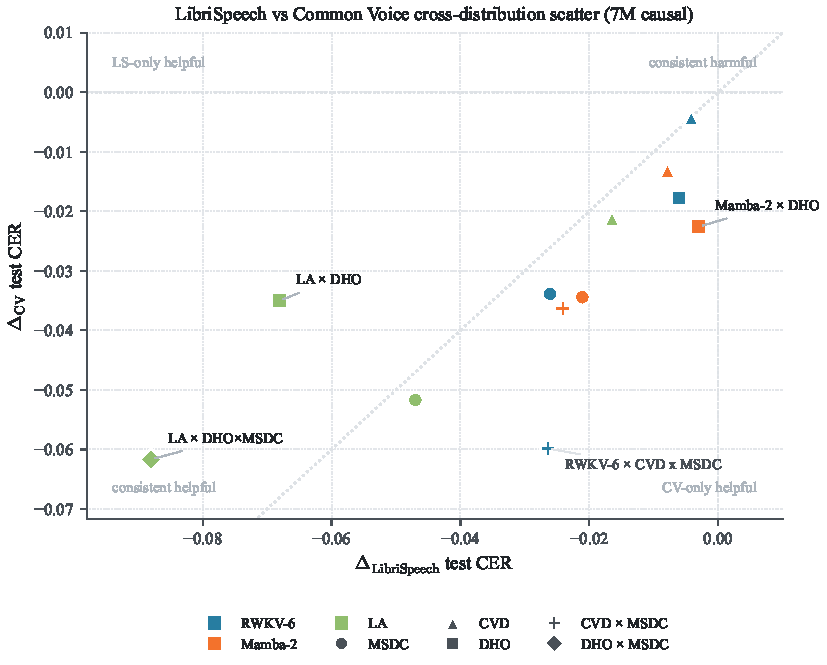
\includegraphics[width=0.9\linewidth]{figures/chapter5/F4_libri_cv_scatter.pdf}
\caption[LibriSpeech versus Common Voice scatter]{Test
$\Delta_{\mathrm{CV}}$ versus $\Delta_{\mathrm{LS}}$ for every
non-vanilla cell at the 7M causal scale. Cells on the diagonal
indicate consistent transfer across the two acoustic
distributions; off-diagonal cells indicate task-prior
modulation. The Mamba-2~$\times$~DHO cell, near the noise floor
on LibriSpeech ($-0.0030$), becomes productive on Common Voice
($-0.0226$).}
\label{fig:f4-libri-cv}
\end{figure}

Twelve of fifteen non-vanilla cells transfer to Common Voice
with $|\Delta_{\mathrm{CV}} - \Delta_{\mathrm{LS}}| < 0.020$,
preserving the rank ordering of the LibriSpeech mechanism
column. Three cells off-diagonal carry the cross-distribution
information of the section. The Mamba-2~$\times$~DHO cell, a
near-null on LibriSpeech, becomes productive on Common Voice
($\Delta_{\mathrm{CV}} - \Delta_{\mathrm{LS}} = -0.0196$): the
selective $\Delta t$ absorption of the block-complex extension
identified in Section~\ref{sec:experiments:transfer} is not
absolute but task-prior modulated, with Common Voice's broader
speaker, accent, and recording-condition variability leaving
residual axis-1 sub-structure that the block-complex extension
exercises. The LA~$\times$~DHO and LA~$\times$~DHO~$\times$~MSDC
cells deliver smaller absolute gains on Common Voice than on
LibriSpeech ($\Delta_{\mathrm{CV}} - \Delta_{\mathrm{LS}} =
+0.0331$ and $+0.0263$), reflecting the absorbed share of the
LA-on-LibriSpeech BREAK pattern under the broader Common Voice
distribution. The RWKV-6~$\times$~CVD~$\times$~MSDC composition
shows the largest amplification in the opposite direction
($\Delta_{\mathrm{CV}} - \Delta_{\mathrm{LS}} = -0.0335$),
consistent with the multi-dilation receptive-field configuration
matching the broader Common Voice phonetic coverage. The reading
refines the alignment criterion: alignment is between mechanism and
\textit{task-as-exercised-by-data} rather than between mechanism
and architecture in isolation.

\section{Axis-2 isolation via MQAR}\label{sec:experiments:mqar}

The Multi-Query Associative Recall benchmark
of~\citet{arora2023zoology} isolates axis~2 by construction:
the sequence comprises $(k, v)$ pairs followed by query keys
whose values must be retrieved, and the difficulty parameter
scales with the ratio of stored pairs $K$ to architectural
state dimension $d$. The cohort sweeps
$T \in \{64, 256, 1024\}$ with the matching
$K \in \{16, 64, 256\}$ across thirteen backbones; verdicts and
convergence speed are reported in
Table~\ref{tab:results:mqar-cohort}. The verdict convention is
the one introduced in Section~\ref{sec:experiments:framework}:
PASS denotes per-sequence accuracy $\ge 0.99$ at the
early-stopping point, PARTIAL denotes $\ge 0.5$ but $< 0.9$ at
the wall-clock budget, and FAIL denotes accuracy at or near zero
with the loss flat near the initialisation level. The
SKIP$^{\dagger}$ marker denotes a cell that was not run because
the same architecture FAILed at a shorter length, since adding
distractors to a non-converging configuration cannot produce
convergence; OOM denotes a cell that exceeded the configured
chunk-size memory budget. The asterisk on the Linear Attention
vanilla $T = 64$ cell marks the partial-but-not-converging case:
the cell reaches $0.5$ per-sequence accuracy at $17$ kS without
reaching $0.9$ within the budget.

\begin{table}[!htbp]
\centering
\small
\caption[MQAR cohort verdicts and convergence speed]{MQAR cohort
verdicts and convergence speed across three sequence lengths.
Each cell reports the per-sequence-accuracy verdict and the
steps-to-0.9 count in thousand-step units (kS) where defined.
Verdict semantics, the SKIP$^{\dagger}$ propagation rule, and
the asterisk on the LA vanilla $T = 64$ cell are described in
the prose around the table.}
\label{tab:results:mqar-cohort}
\setlength{\tabcolsep}{6pt}
\renewcommand{\arraystretch}{1.15}
\begin{tabularx}{\linewidth}{@{}X c c c@{}}
\toprule
\textbf{Backbone} & \textbf{$T = 64$} & \textbf{$T = 256$} & \textbf{$T = 1024$} \\
\midrule
Causal Transformer       & PASS / 5 kS  & PASS / 12 kS & \textbf{FAIL} \\
\addlinespace
RWKV-6                   & FAIL          & FAIL          & SKIP$^{\dagger}$ \\
RWKV-6 + MSDC            & PASS / 4 kS  & PASS / 3 kS  & PASS / 2 kS \\
RWKV-6 + CVD             & PASS / 6 kS  & PASS / 3 kS  & PASS / 4 kS \\
RWKV-6 + DHO             & FAIL          & SKIP$^{\dagger}$ & SKIP$^{\dagger}$ \\
\addlinespace
Mamba-2                  & FAIL          & FAIL          & SKIP$^{\dagger}$ \\
Mamba-2 + MSDC           & PASS / 2 kS  & PASS / 1 kS  & PASS / 1 kS \\
Mamba-2 + CVD            & PASS / 5 kS  & PASS / 3 kS  & PASS / 2 kS \\
Mamba-2 + DHO            & FAIL          & SKIP$^{\dagger}$ & SKIP$^{\dagger}$ \\
\addlinespace
Linear Attention         & PARTIAL$^{\ast}$ & FAIL          & SKIP$^{\dagger}$ \\
Linear Attention + MSDC  & PASS / 6 kS  & PASS / 4 kS  & PASS / 5 kS \\
Linear Attention + CVD   & PASS / 2 kS  & PASS / 2 kS  & PASS / 3 kS \\
Linear Attention + DHO   & FAIL          & SKIP$^{\dagger}$ & OOM \\
\bottomrule
\end{tabularx}
\end{table}

\paragraph{Linear-time plus mechanism solves MQAR at every
tested length.} Vanilla RWKV-6, Mamba-2, and Linear Attention
all FAIL or PARTIAL at $T = 64$ already, confirming the
no-recall baseline of the diagonal class without explicit
interference cancellation. Adding MSDC or CVD to any of the
three backbones sends the cell to PASS at every tested length,
in one to six thousand training steps. The causal Transformer
baseline PASSes at $T = 64$ and $T = 256$ within twelve
thousand steps but \textit{FAILs at $T = 1024$}. The mechanism
behind the FAIL is structural: at $T = 1024$ with $K = 256$, the
model must learn an induction-head-like
circuit~\cite{olsson2022induction} that selects one of $256$
stored keys against $T - K = 768$ distractor positions per query.
The gradient signal for forming such a circuit weakens as $K$
grows, since the softmax distribution diffuses across the larger
key population before a length-aware attention pattern
stabilises; vanilla causal attention with sinusoidal positional
encoding does not converge on the task within the matched
30-thousand-step budget, and the same degradation pattern is the
central observation of the original Zoology
study~\cite{arora2023zoology}. The mechanism-augmented
linear-time backbones bootstrap the task by construction: MSDC
supplies short-range mixing that produces consistent local
representations early in training, and CVD applies a chunk-local
key-similarity preconditioner that cancels interference before
values enter the recurrence, short-circuiting the
circuit-formation cost that vanilla causal attention pays
implicitly. The empirical result inverts the standard
sub-quadratic-versus-quadratic narrative at the sequence length
where the comparison becomes binding.

\paragraph{DHO does not solve MQAR.} Every DHO cell in the
cohort FAILs at $T = 64$ already, with the Linear Attention DHO
cell additionally exceeding the configured chunk-size memory
budget at $T = 1024$. The pattern is the predicted axis
mismatch from Section~\ref{sec:axes}: DHO extends the function
class along axis~1, the damped-oscillator sub-axis; MQAR
exercises axis~2, associative-memory capacity under
interference. A mechanism that extends the function class along
axis~1 does not convert into measured gain on a task that
exercises axis~2, regardless of how productively it transfers
on the matched-axis probe.

\section{Composition behaviour}\label{sec:experiments:composition}

The pre-registered composition cells of the matrix probe whether
mechanism-prior alignment extends to pairs of mechanisms applied
jointly. The matrix populates one productive composition (the LA
DHO~$\times$~MSDC stack, which couples a phase-side and an
input-side mechanism on the backbone with the largest residual
deficit), one composition that saturates to single-mechanism level
(CVD~$\times$~MSDC on RWKV-6, where CVD's value-decorrelation
contribution intersects the residual deficit MSDC already
addresses), and one that stacks marginally
(CVD~$\times$~MSDC on Mamba-2). Figure~\ref{fig:f6-composition}
shows the pattern across the matrix. The reading is directional
rather than a closed-form composition rule, since only three
composition cells are populated.

\begin{figure}[!htbp]
\centering
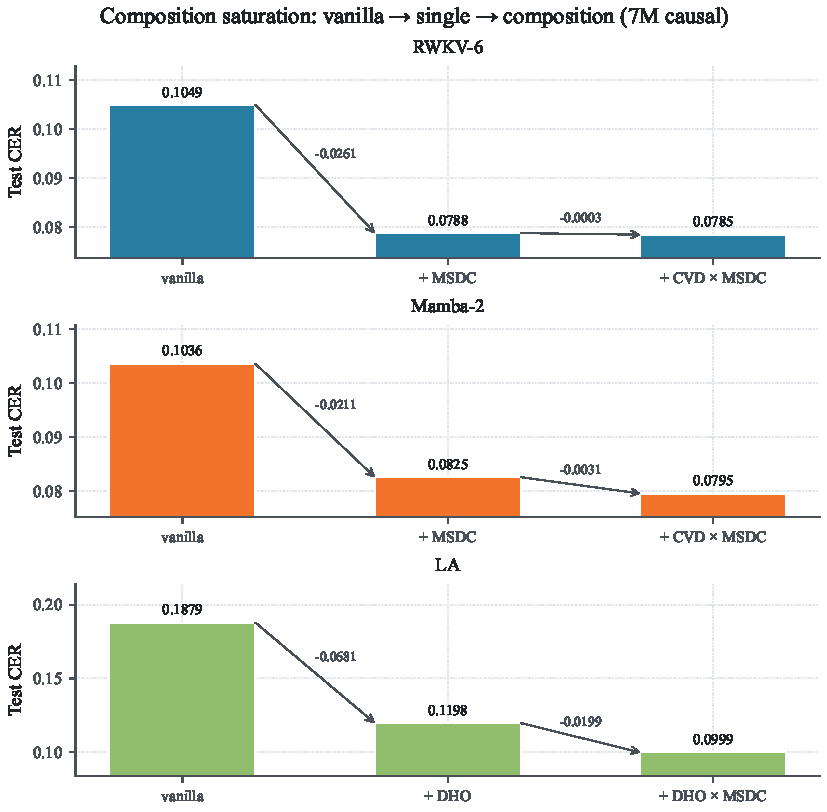
\includegraphics[width=0.9\linewidth]{figures/chapter5/F6_composition_saturation.pdf}
\caption[Composition saturation pattern]{Vanilla, best single
mechanism, and pre-registered composition test character error
rate per architecture and scale on the causal matrix. Bars
within each (architecture, scale) group are ordered vanilla
$\to$ best single mechanism $\to$ composition. Composition
saturates to single-mechanism level on RWKV-6, stacks marginally
on Mamba-2, and stacks productively on Linear Attention.}
\label{fig:f6-composition}
\end{figure}

The CVD~$\times$~MSDC composition pre-registered on RWKV-6 and
Mamba-2 saturates on RWKV-6 ($\Delta$ over MSDC alone:
$-0.0003$ at 7M, $-0.0005$ at 14M) and stacks marginally on
Mamba-2 ($-0.0030$ at 7M, $-0.0013$ at 14M); the Mamba-2
advantage is consistent with CVD's stronger single-mechanism
transfer on Mamba-2 than on RWKV-6
(Section~\ref{sec:experiments:transfer}). The matrix ceiling at
14M Mamba-2 falls on this composition cell at test $0.0618$.
The DHO~$\times$~MSDC composition pre-registered on Linear
Attention stacks productively at both scales: at 7M causal,
$\Delta = -0.0410$ over MSDC alone, since MSDC fills the
absent input-side mixing deficit and DHO independently fills
the absent transition-side phase deficit; at 14M the
composition delivers $\Delta = -0.0183$ over MSDC alone. The
contrast between the saturating CVD~$\times$~MSDC composition on
RWKV-6 and the productive DHO~$\times$~MSDC composition on
Linear Attention is structural: composition stacks where the
two mechanisms target distinct deficits on the architecture's
operator chain, and saturates where the second mechanism
intersects the deficit the first already addresses.

\section{Convergence under matched budget}\label{sec:experiments:convergence}

The matched 50-epoch training budget supports the
matrix-as-artefact framing only if every reported cell
converges within its horizon; otherwise an apparent gain or
loss might reflect budget truncation rather than the
underlying mechanism's structural reach.
Figure~\ref{fig:f11-training-curves} plots dev character error
rate against epoch for every cell of the matrix.

\begin{figure}[!htbp]
\centering
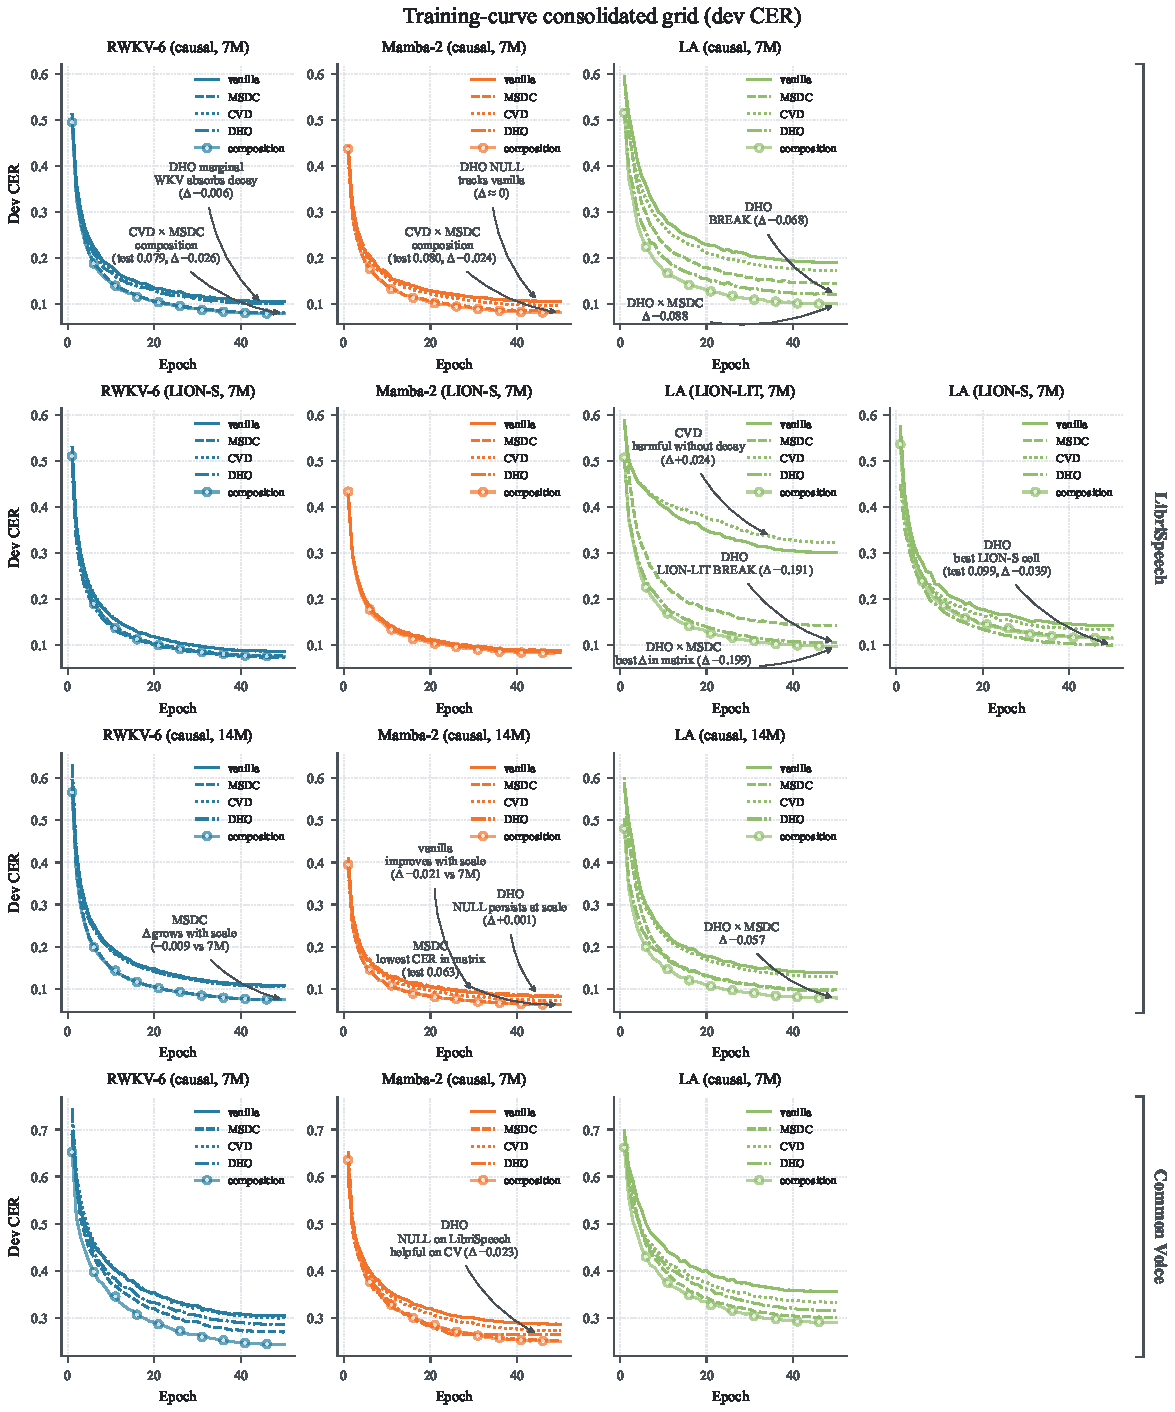
\includegraphics[width=0.9\linewidth]{figures/chapter5/F11_training_curves.pdf}
\caption[Per-cell training curves]{Dev character error rate
versus epoch across every cell of the matrix at 7M and 14M
causal modes, the 7M LION mode, and the 7M Common Voice pilot.
Lines are styled by mechanism: vanilla solid, MSDC dashed, CVD
dotted, DHO dash-dot, composition solid with markers. The
patience-15 early-stopping criterion is not triggered for any
reported cell within the 50-epoch horizon.}
\label{fig:f11-training-curves}
\end{figure}

Two structural callouts on the 14M causal block confirm that
the matrix endpoints are structural rather than budget-limited.
The 14M RWKV-6 vanilla curve plateaus at the matched budget
with slope close to zero, falsifying an undertraining-at-14M
hypothesis: the architecture-specific NEG-scaling on RWKV-6
vanilla ($\Delta = +0.0054$ on the 7M-to-14M comparison) is
structural rather than a consequence of insufficient training.
The 14M Mamba-2 MSDC curve plateaus at $0.063$ with similar
near-zero slope at the final epoch, confirming that the matrix
ceiling is reached within the matched budget rather than by
exhaustion of available training time.

\section{Synthesis: mechanism-prior alignment}\label{sec:experiments:synthesis}

The matrix supports a predictive criterion that we call
mechanism-prior alignment: a mechanism's gain on a task is
proportional to the residual structural deficit the
architecture leaves uncovered along the axis the mechanism
targets, and is null when the mechanism's axis is not
exercised by the task. Six structural signatures from the
chapter populate the criterion.

Three signatures sit on the cross-architecture transfer row.
The MSDC mechanism transfers in deficit-proportional ordering
across the family (LA $>$ RWKV-6 $>$ Mamba-2 at both scales),
matching the architecture-deficit map of
Section~\ref{sec:backbones:deficit}. The DHO mechanism
delivers a structural BREAK on Linear Attention and a
near-null on Mamba-2 under the LibriSpeech distribution,
matching the prediction that the block-complex extension's
reach is largest on the architecture with no native
attenuation and no native phase. The CVD mechanism transfers
asymmetrically across the family, opposite to a
natural-home-in-attention prior.

A controlled falsifier sharpens the bidirectional reading: the
LION-LIT~$\times$~CVD cell on Linear Attention is the single
positive $\Delta$ in the matrix and isolates decay as the
structural prerequisite for the value-decorrelation mechanism
in the bidirectional setting, while the controlled LION-S
deployment restores productive transfer.

A cross-distribution refinement adjusts the criterion: the
Mamba-2~$\times$~DHO cell, marginal on LibriSpeech and
productive on Common Voice, indicates that alignment is between
mechanism and \textit{task-as-exercised-by-data} rather than
between mechanism and architecture in isolation.

The axis-2 isolation closes the loop. On the MQAR length sweep,
mechanism-augmented linear-time backbones solve the task at
every tested length while the causal Transformer FAILs at
$T = 1024$; the DHO cells FAIL at $T = 64$ already, matching
the predicted axis mismatch between an axis-1 mechanism and
an axis-2 task.

\paragraph{One-directional matrix evidence.} The six signatures
above populate the positive-transfer half of the criterion: where
a mechanism's axis is exercised by the task, gain materialises in
the predicted ordering. The converse half, where a mechanism
engages under stochastic gradient descent without converting into
measured task gain, is not exercised by the matrix and is left to
the discovery-phase archive that preceded the 50-epoch budget.
The matrix evidence reported in this chapter is therefore
one-directional with respect to the criterion; the
falsification-protocol extension recorded in
Section~\ref{sec:conclusions:future-work} of
Chapter~\ref{ch:conclusions} commits the framework to a
two-directional protocol as future work.

\paragraph{Scope.} The criterion as stated holds within the
diagonal-class function family of
Section~\ref{sec:bounds}. The matrix does not test it on
diagonal-plus-low-rank architectures, and the criterion is
not asserted there. The natural extension of the framework is
to repeat the cross-architecture transfer matrix on a
diagonal-plus-low-rank backbone class such as
DeltaNet~\cite{schlag2021deltanet, yang2024deltanet} or
RWKV-7~\cite{peng2025rwkv7}, with mechanisms targeting axis~3
(non-Abelian state-tracking).
Chapter~\ref{ch:conclusions} returns to this extension as the
principal future-work direction.
